% pdf/a 
\begin{filecontents*}[overwrite]{\jobname.xmpdata}
    \Title{Rádióátviteli mérések laboratórium 2, 10. mérés}
    \Author{Szilágyi Gábor}
    \Language{hu-HU}
    \Subject{ADS-B jel vétele}
    \Keywords{ADS-B, OOK, Manchaster-kód, valósidejű jelfeldolgozás}
    \Publisher{Szilágyi Gábor}
\end{filecontents*}

\documentclass[a4paper,12pt,titlepage]{article}
%\documentclass[a4paper,12pt,titlepage,draft]{article}
\usepackage{ucs}
\usepackage[T1]{fontenc}
\usepackage[utf8]{inputenc}
\usepackage[magyar]{babel}
\usepackage{amsfonts}
\usepackage{amsmath,bm}
\usepackage{amssymb}
\usepackage{graphicx}
%\usepackage[hang]{caption}
\usepackage{subcaption}
%\usepackage{blkarray,booktabs,bigstrut} % a címkézett mátrixhoz
%\usepackage{enumerate}
%\usepackage{psfrag}
\usepackage[left=25mm,right=25mm,top=25mm,bottom=25mm]{geometry}
%\usepackage[hyphenbreaks]{breakurl}
%\usepackage[hyphens]{url}
%\usepackage{multirow}
%\usepackage{booktabs}
%\usepackage{hyperref}
\usepackage{listings}
%\usepackage{cite}
%\usepackage{csquotes}
\usepackage{siunitx}
\usepackage{xcolor}
\usepackage[a-3u]{pdfx}
\hypersetup{
    colorlinks,
%    linkcolor={red!50!black},
    linkcolor={black},
%    citecolor={blue!50!black},
    citecolor={black},
%    urlcolor={blue!80!black}
    urlcolor={blue!80!black}
}

\definecolor{mygray}{RGB}{240, 240, 240}
\definecolor{mygreen}{RGB}{0, 140, 40}

\lstset{ % General setup for the package
	language=C,
	basicstyle=\scriptsize\ttfamily,
	numbers=left,
	numberstyle=\tiny,
	tabsize=4,
	backgroundcolor=\color{mygray},
	columns=fixed,
	showstringspaces=false,
	showtabs=false,
	keepspaces,
	frame=trbl,
	breaklines=true,
	%breakwhitespace=true,
	morekeywords={sort2,sort8},
	stringstyle=\color{red},
	commentstyle=\color{mygreen},
	keywordstyle=\color{blue}
}

\sisetup{
    range-phrase=--,
    range-units=single,
    output-decimal-marker={,},
    tight-spacing=true,
    print-unity-mantissa=false,
}

%\DeclareMathOperator{\exp}{exp}
%\DeclareMathOperator{\rot}{rot}
%\DeclareMathOperator{\min}{min}
%\DeclareMathOperator{\divergence}{div}

\sloppy % Margón túllógó sorok tiltása.
\widowpenalty=10000 \clubpenalty=10000 %A fattyú- és árvasorok elkerülése
\def\hyph{-\penalty0\hskip0pt\relax} % Kötőjeles szavak elválasztásának engedélyezése

\frenchspacing
\pagestyle{plain} 

%\listfiles % a package-ek kilistázása a logba

\title{
    \centering
    
\includegraphics[width=0.48\textwidth]{kep/bme_logo.pdf} \\
    \vspace{0.5cm}
    \large{\bf Budapesti Műszaki és Gazdaságtudományi Egyetem \\
    Villamosmérnöki és Informatikai Kar \\
    Szélessávú Hírközlés és Villamosságtan Tanszék}\\
    \vspace{0.5cm}
    
\includegraphics[width=0.3\textwidth]{kep/hvt_logo.png} \\
    \vspace{3cm}
    \large{Rádióátviteli mérések laboratórium 2} \\
    \vspace{2cm}
    \Large{\bf{10. mérés\\ADS-B vétel}} \\
    \vspace{2cm}
}

%\parskip=10pt
%\parindent=0pt

%\newcommand\adj[1]{#1^{\mathrm{H}}}

\author{Szilágyi Gábor \hspace{1cm} NOMK01}
\date{Budapest, \today}


\begin{document}
%
\maketitle
\setcounter{page}{2}
\section{A feladat}
    Erre a laboralkalomra a feladat egy C program kiegészítése, ami készen alkalmas arra, hogy valós időben egy szoftverrádióból érkező mintákból dekódolja az ADS-B adásokat. Tanszéki számítógépes terem hiányában konzerv fájlokból kellett kihámoznunk az előre felvett adásokat. A feladathoz nagy segítség a rendelkezésre álló programkód-váz (\ref{adsb.c} függelék), ezt kellett kiegészíteni a minták feldolgozását végző és az eredményeket kiíró résszel.
\section{A megoldás lépései}
    \subsection{OOK kódolt bitek előállítása}
        A bejövő I/Q mintákból először amplitúdót számolok. Ehhez egy előre elkészített, 128-as referenciaszinthez igazított look up table áll rendelkezésre, amiből egyszerűen ki kell olvasni az adott I és Q értékekhez tartózó amplitúdót. Erre azért van szükség, mert mintánként egyesével újraszámolni az amplitúdót a gyökvonás miatt túl költséges lenne a megadott mintavételi frekvencia mellett.

        Az amplitúdókból egy FIR szűrővel mozgó átlagot állítok elő, a szűrőablak \verb|FIR_LEN = 8| minta hosszú. Erre a lépésre azért van szükség, hogy különböző vételi teljesítményű jelek esetén is helyesen el lehessen végezni a 0/1 döntést. A FIR szűrő egy egyszerű mozgóátlag, így a késleltetése \verb|FIR_LEN/2 = 4| minta hosszú, tehát ennyivel a legújabbnál régebbi mintára vonatkozó mozgóátlagot állít elő. Az eredeti I/Q minták (,,I'' és ,,Q''), az amplitúdó (,,Abs'') és a belőle képzett mozgóátlag (,,Avg'') \aref{fig:signals}. ábrán láthatóak. A szűrőhöz szükséges késleltetés egy cirkuláris buffer segítségével van megvalósítva, az átlagképzéshez pedig egy akkumulátort használok és az átlag \verb|FIR_LEN|-szeresét tárolom, így itt sincs szükség mintánként egy osztásra, csak egy összeadásra, egy kivonásra és memóriaírásra, ill. -olvasásra.
        \begin{figure}
            \centering
            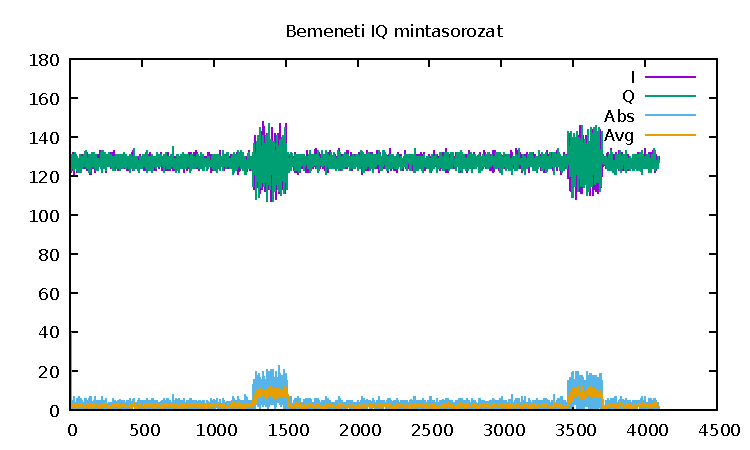
\includegraphics[width=\textwidth]{kep/signals.pdf}
            \caption{A konzerv fájlból kiolvasott I/Q minták, az amplitúdó és az amplitúdó mozgóátlaga.}
            \label{fig:signals}
        \end{figure}

        A mozgóátlagot az OOK modulációnál adaptív döntési szintként lehet használni, ami az ON és OFF teljesítményszintek átlaga közelébe áll be, ha a 0-s és 1-es bitek gyakorisága körülbelül megegyezik. A Manchaster kódolásnál ez automatikusan teljesül. Az aktuálisan feldolgozott (4 ütemmel ez előtti) minta amplitúdóját a legutóbb kiszámolt átlagszinthez komparálom, ez alapján döntök 0-s vagy 1-es bitre. Pontosabban az aktuális LUT-ból kiolvasott amplitúdó \verb|FIR_LEN|-szeresét számolom ki és ezt hasonlítom össze az akkumulátorban tárolt értékkel, ami az átlag \verb|FIR_LEN|-szerese. Így ennél a lépésnél sincs szükség minden ütemben osztás műveletet végezni. Mivel a mintavételi sebesség megegyezik a bitsebsséggel, minden bejövő mintából egy bit áll elő.
    \subsection{Állapotgép a bitek feldolgozásához}
        Az aktuális bit segítségével vezérlek egy állapotgépet. Ennek az első feladata az ADS-B adás premble-jének felismerése, amely 16 bit hosszú. Itt egyszerűen egy számlálóval a preamble megadott mintázatával egyező előző biteket számolom. Ha az aktuális bit hibás, akkor nullázom a számlálót és elölről kezdem a keresést. Ha a számláló elért 16-ig, akkor ez azt jelenti, hogy megtaláltam a preamble-t, következik még 112 adatbit, ami a Manchaster-kódolás miatt 224 bitet jelent, így összesen 240-ig kell elszámolni. A Manchaster-dekódoláshoz egyszerűen a kód bitpárjaiból az első bit adja meg az adatbitet (0-tól indexelve így a páros indexű bejövő bitek).

        Az adatbitek kiírásához 8-asával bájtokba rendezem őket, majd a hexadecimális értékeket kiírom a kimenetre. A megtalált adások elejét új sorral és csillaggal jelzem. A teljes konzervfájlra a kimenet \aref{test.txt}. függelékben olvasható. A kimenet első sorának utolsó 4 karaktere (\verb|6186|) megegyezik a bemeneti mintákat tartalmazó fájl nevében megadott részlettel, ebből látszik, hogy a dekódolás helyes. Az ábrák generálásához a Gnuplot programot használtam, aminek az ábrát generáló szkriptje \aref{plotter.gp}. függelékben látható.
%\bibliography{mybib}
%\bibliographystyle{plain}
%
\clearpage
\appendix
%
\section{test.txt (dekódolt adat)}
    \label{test.txt}
	\lstinputlisting{code/test.txt}
\section{build}
	\lstinputlisting{code/build}
\section{run}
	\lstinputlisting{code/run}
\section{plotter.gp}
    \label{plotter.gp}
	\lstinputlisting{code/plotter.gp}
\section{adsb.c}
    \label{adsb.c}
    \lstinputlisting{code/adsb.c}
%
\end{document}

%\cite{Henneron14}

%            \begin{align}
%                \label{equ:svd}
%                {\bf S}~=&~{\bf U \Sigma \adj{V}}
%            \end{align}

%            \begin{figure}
%                \centering
%                \includegraphics[width=0.8\textwidth]{kep/szerkesztett/wstk-mighty-gecko-nagy.jpg}
%                \caption{WSTK + radio board.}
%                \label{fig:wstkmighty}
%            \end{figure}
% \cite{Anritsu}
%            \begin{figure}
%                \centering
%                \begin{subfigure}{0.48\textwidth}
%                    \includegraphics[width=\textwidth]{kep/szerkesztett/sol-868-conducted.png}
%                    \caption{\SI{868}{MHz}}
%                \end{subfigure}
%                \begin{subfigure}{0.48\textwidth}
%                    \includegraphics[width=\textwidth]{kep/szerkesztett/sol-470-conducted.png}
%                    \caption{\SI{470}{MHz}}
%                \end{subfigure}
%                \caption{470 és \SI{868}{MHz}-es Sol radio board-ok kimeneti spektruma.}
%                \label{fig:sol-conducted}
%            \end{figure}

